\documentclass{article}
\usepackage{amsmath}
\usepackage{amsthm}
\usepackage{amsfonts}
\usepackage{amssymb}
\usepackage{tikz-cd}
\date{\vspace{-10ex}}
\begin{document}
$ $ \\
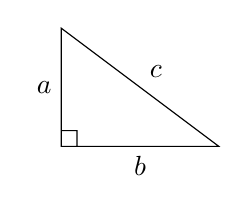
\begin{tikzpicture}
\draw (0, 0) node{}
  -- (0, 1.5) node[midway, left]{$a$}
  -- (2, 0) node[midway, above right]{$c$}
  -- (0, 0) node[midway, below]{$b$}
  -- (0, .2) node{}
  -- (.2, .2) node{}
  -- (.2, 0) node{};
\end{tikzpicture} \\
$a^2 + b^2 = c^2$

$ $\\

$ $\\

$ $\\

$ $ \\
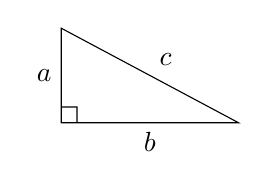
\begin{tikzpicture}
\draw (0, 0) node{}
  -- (0, 1.2) node[midway, left]{$a$}
  -- (2.25, 0) node[midway, above right]{$c$}
  -- (0, 0) node[midway, below]{$b$}
  -- (0, .2) node{}
  -- (.2, .2) node{}
  -- (.2, 0) node{};
\end{tikzpicture} \\
\phantom{30}\phantom{30}$a^2 + b^2 = c^2$
\end{document}